% ======================================================================
% Annual Meeting Paper Template
% Updated for the supplied requirements and Word template.
% ======================================================================

% Document class selection. Leave \manuscriptclass empty to auto-check for a
% .cls file. Auto mode uses a .cls file matching this manuscript name when
% available, then falls back to trbunofficial.cls. If multiple .cls files are
% available, enter the intended class name without the .cls extension.
\newcommand{\manuscriptclass}{}
\newcommand{\selectedmanuscriptclass}{}
\makeatletter
\ifx\manuscriptclass\@empty
  \IfFileExists{\jobname.cls}{%
    \renewcommand{\selectedmanuscriptclass}{\jobname}%
  }{%
    \IfFileExists{trbunofficial.cls}{%
      \renewcommand{\selectedmanuscriptclass}{trbunofficial}%
    }{%
      \PackageError{trb_template}{No document class file found}{%
        Add a .cls file that matches this manuscript file name, add
        trbunofficial.cls, or set \string\manuscriptclass\space to the class
        name explicitly.%
      }%
    }%
  }%
\else
  \renewcommand{\selectedmanuscriptclass}{\manuscriptclass}%
\fi
\makeatother

% Change 10pt to 11pt or 12pt only if your target venue allows it.
\documentclass[10pt,numbered]{\selectedmanuscriptclass}

\begin{document}

% Use \numberedblankline when a visible blank line should also receive a
% line number.

% ---------- Title Page ----------
\title{Title of Paper Format Example}

% The title should capitalize the first letter of each major word, except
% conjunctions, prepositions, and articles.

% Use \author* for the corresponding author and \author otherwise.
% \author*{Name}{Job title}{Institutional affiliation}{Email}[Address][ORCID]
\author*{Xiangyong Luo}{Academic Position}{Department of XXX, Institution Name}{author@university.edu}[City, State or Country, Postcode][https://orcid.org/0000-0000-0000-0000]

\author{Public Sector Author Name}{Position}{State Department of Transportation, Department if Applicable}{abc@dot.gov}[City, State or Country, Postcode]

\author{Private Practitioner Author Name}{Position}{Company Name}{enj@abc.com}[City, State or Country, Postcode]

% Submission date appears on the title page. Leave the braces empty to use
% today's date, enter a date to override it, or comment out the next line if
% this line is not needed.
\submissiondate{}

% Total Number of Pages appears on the title page. Leave the braces empty to
% calculate the page count automatically, enter a number to override it, or
% comment out the next line if this line is not needed.
\totalpages{}

% Optional title-page footnote. Edit the text inside the braces, add another
% \titlefootnote{...} line for an additional note, or comment out this line if
% no title-page footnote is needed.
\titlefootnote{Length: The length of each paper, including the title page, structured abstract, text, acknowledgments, references, figures, and tables, must not exceed 20 pages. Papers not meeting this requirement may be withdrawn from the review process at any time. The paper submission system, Editorial Manager, will generate its own cover page, which does not count toward the page limit.
Page size and margins: 8.5x11 inch page with 1 inch margins
Font: Times New Roman font, 10 pt size
Spacing: single spaced
Columns: single column
Line numbering: line numbering is required with line numbers restarting at 1 on each page
Page numbers: pages must be numbered with page numbers centered at the bottom of each page
Tables and figures should be embedded in the text, near the text that discusses the item
Supplemental Material/Appendices are not permitted in TRB Annual Meeting papers.
References should be called out
Front Matter
Title page with: paper title; job titles, institutional affiliations, and email addresses; and total number of pages. Note: you will also be required to enter this information into Editorial Manager when you submit. ORCiD numbers are optional, but strongly encouraged.
The title should have the first letter of each word capitalized, except for conjunctions, prepositions, and articles.
Structured abstracts must meet length and content requirements  The structured abstract replaces the traditional
 Structured Abstract
To facilitate the initial screening of your paper and direct papers more quickly to appropriate reviewers, manuscripts must include a structured abstract that clearly and concisely summarizes the objectives, methodology, principal findings, and contribution of the research. The structured abstract also facilitates Annual Meeting attendees’ ability to quickly identify papers of interest to them. The structured abstract replaces the traditional (unstructured) abstract. Structured abstracts must conform to the requirements below. An example of a structure abstract can be found in the sample papers.}

\maketitle

% ---------- Structured Abstract ----------
% Required headings, in order: Objectives, Methods, Findings, Novelty,
% Practical Applications. Keep the full structured abstract to 300 words or
% fewer. Do not include figures, tables, equations, or undefined acronyms.
\section*{ABSTRACT}

\begingroup
\setlength{\parindent}{0pt}

\numberedblankline
\noindent\textbf{Objectives:} Fare capping, a policy in which a transit agency
caps the maximum amount a rider pays over a given period, has emerged as a
recent innovation in public transit fare policy. The objective of this research
is to compile and compare fare capping policies across U.S. transit agencies
and to explore potential rider benefits.

\par\numberedblankline
\noindent\textbf{Methods:} A multiple case study method was used to examine fare
capping policies at the 101 largest transit agencies in the United States.
Agency fare policies were identified through publicly available documents, and
daily, weekly, and monthly caps were coded for each agency. The analysis
calculated the number of one-way adult fares required to reach each cap and
compared the resulting discount patterns.

\par\numberedblankline
\noindent\textbf{Findings:} As of September 2021, fare capping was adopted by at
least 21 of the 101 largest U.S. transit agencies. Most daily fare caps offered
little discount for a typical two-trip commuter, but daily caps provided more
meaningful discounts to transit-dependent riders, tourists, and other frequent
riders.

\par\numberedblankline
\noindent\textbf{Novelty:} This paper provides one of the first systematic
syntheses of fare capping policies across major U.S. transit agencies. It also
introduces a comparative framework based on cap structure, trip thresholds, and
rider discount levels.

\par\numberedblankline
\noindent\textbf{Practical Applications:} The findings can help transit agencies
design fare capping policies that better match rider travel patterns and policy
goals. Agencies can use the framework to compare operational contexts, equity
goals, and implementation constraints.
\par\endgroup
\newpage

% ---------- Main Text ----------
\section{Introduction}\label{sec:intro}
Sed efficitur magna nisl, id aliquet leo molestie et. Quisque vestibulum
imperdiet neque, id cursus felis rutrum et. Duis porttitor nisl arcu, sit amet
varius justo convallis vitae. Maecenas pretium ullamcorper massa sed volutpat
\citep{smith2020}. Duis libero augue, porttitor sed magna quis, ultrices
molestie magna. Nam in orci in dolor accumsan rhoncus ut et leo. Phasellus
rutrum enim ut purus lacinia, eget faucibus odio fermentum.

Morbi dictum placerat erat ac tempor. Pellentesque elementum accumsan quam.
Integer ultricies feugiat placerat. Morbi quis eros et augue iaculis auctor.
Aliquam rhoncus lacus ut tortor egestas, in luctus nisl semper. Quisque
ultrices sapien turpis, at aliquam est sodales sit amet. Nulla congue risus in
ligula aliquam cursus.

\section{Methods}
Mauris scelerisque maximus viverra. Proin sagittis faucibus viverra. Ut et
tellus eros. Mauris sollicitudin porttitor enim vel congue. Quisque dictum
ornare posuere. Fusce malesuada rhoncus nisl sit amet rutrum. Vivamus posuere
elit dui, eu scelerisque urna interdum sed.

Duis ut turpis maximus, semper sapien in, elementum metus. Proin sit amet sem
sit amet tortor blandit dapibus. Nam fringilla nunc quis nisl faucibus laoreet.
Nam eu elit laoreet, iaculis sem quis, rhoncus libero \citep{smithJones2020}.

\subsection{Level 2 Header}
Quisque ultrices sapien turpis, at aliquam est sodales sit amet. Nulla congue
risus in ligula aliquam cursus. Sed vel augue consequat orci mollis aliquet nec
non arcu. Sed scelerisque quam elementum, maximus tortor ut, suscipit arcu.

\subsubsection{Level 3 Header}
Fusce malesuada rhoncus nisl sit amet rutrum. Vivamus posuere elit dui, eu
scelerisque urna interdum sed \citep{smithEtAl2020}. Etiam quis libero id
lacus bibendum interdum. Morbi et pretium lorem \citep[25--27]{smith2021}.

\begin{figure}[htbp]
  \centering
  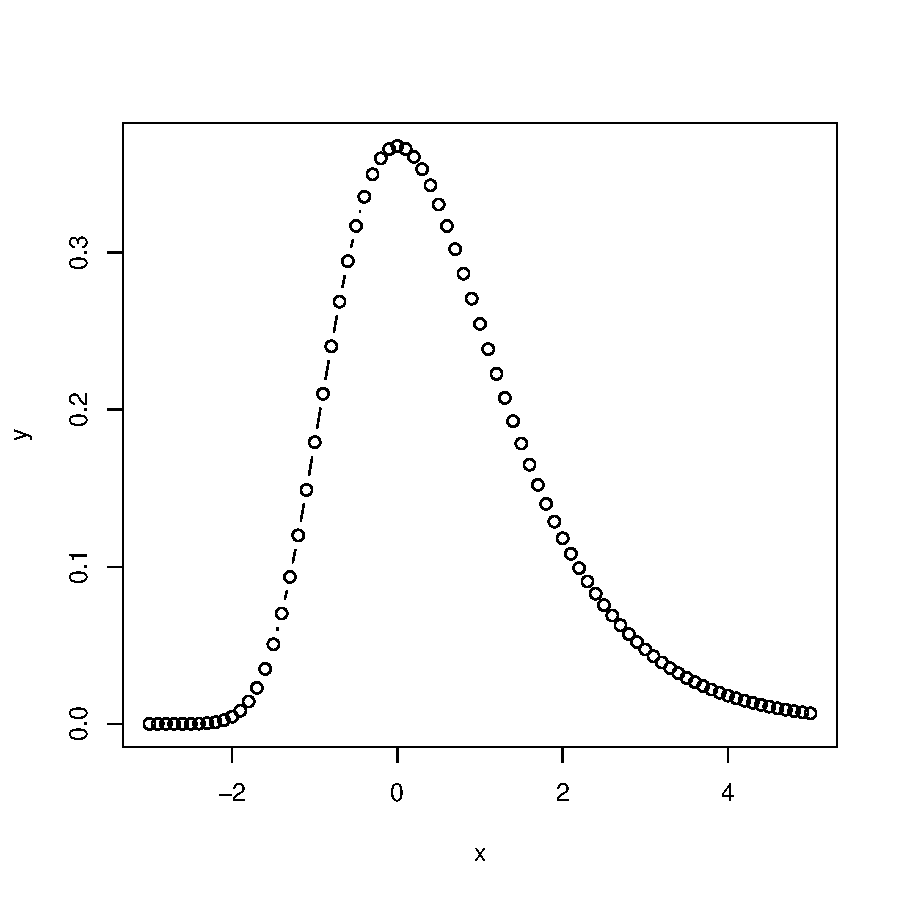
\includegraphics[width=0.55\linewidth]{trb_template-gumbel}
  \caption{Caption for figure}\label{fig:example}
\end{figure}

Maecenas pretium ullamcorper massa sed volutpat. Duis libero augue, porttitor
sed magna quis, ultrices molestie magna. Nam in orci in dolor accumsan rhoncus
ut et leo. Figure~\ref{fig:example} shows the expected placement of figures
near the relevant discussion.

\section{Results}
Nulla eu urna et erat bibendum venenatis sit amet sed sem. Nam quis quam
tempor, placerat turpis a, imperdiet ante. Integer eleifend aliquam magna quis
viverra. Nulla consequat sem vitae mi lacinia maximus.

\begin{table}[htbp]
  \caption{Measurement Conversion}\label{tab:conversion}
  \centering
  \begin{tabular}{lll}
    \hline
    When You Know & Multiply by & To Find \\
    \hline
    inches (in.) & 25.4 & millimeters (mm) \\
    feet (ft) & 0.305 & meters (m) \\
    yards (yd) & 0.914 & meters (m) \\
    miles (mi) & 1.61 & kilometers (km) \\
    acres & 0.405 & hectares (ha) \\
    \hline
  \end{tabular}
\end{table}

Sed eu lacus sit amet risus sodales pretium a ac ex. Donec gravida auctor
efficitur. Curabitur maximus pellentesque mollis. Table~\ref{tab:conversion}
shows an example table embedded near the text that discusses it.

\section{Discussion}
Nunc eros felis, dapibus eu nisl convallis, pellentesque facilisis sapien.
Duis vel magna ac ligula rutrum volutpat. Donec sed malesuada ipsum. Morbi sed
metus sem. Etiam bibendum posuere elementum.

Equations are left aligned and should be introduced in the surrounding text:
\begin{align}
  \dot{x}_\alpha &= \frac{\mathrm{d}x_\alpha}{\mathrm{d}t} = v_\alpha,\\
  \dot{v}_\alpha &= a\!\left[
    1 - \left(\frac{v_\alpha}{v_0}\right)^\delta
    - \left(\frac{s^*(v_\alpha,\Delta v_\alpha)}{s_\alpha}\right)^2
  \right].
\end{align}

Donec libero velit, bibendum sit amet dignissim in, tempus vel lorem. Donec
consectetur dui lorem, gravida eleifend metus blandit ut. Fusce metus lorem,
volutpat sagittis orci id, lobortis semper lectus.

\section{Conclusions}
Nulla eu urna et erat bibendum venenatis sit amet sed sem. Nam quis quam
tempor, placerat turpis a, imperdiet ante. Integer eleifend aliquam magna quis
viverra. Nulla consequat sem vitae mi lacinia maximus.

Supplemental material and appendices are not permitted for this paper format
and should not be included in this manuscript.

\section{Acknowledgments}
The author must be transparent in their use of artificial intelligence (AI) or
large language models in the Submission Details tab in Editorial Manager and,
where appropriate, in this section.

% If generative AI was used to produce or substantially modify content, disclose
% the tool and purpose. Assistive spelling, grammar, punctuation, and basic
% sentence-structure tools do not require disclosure.
% \AIDisclosure{The authors used [tool name and version] to [specific
% purpose]. The authors reviewed and verified all AI-assisted outputs.}

\section{Author Contributions}
The authors confirm contribution to the paper as follows: study conception and
design: X.~Author, Y.~Author; data collection: Y.~Author; analysis and
interpretation of results: X.~Author, Y.~Author, Z.~Author; draft manuscript
preparation: Y.~Author, Z.~Author. All authors reviewed the results and
approved the final version of the manuscript.

\section{Declaration of Conflicting Interests}
% Choose one of the following statements.
The authors declared no potential conflicts of interest with respect to the
research, authorship, and/or publication of this article.

% The authors declared the following potential conflicts of interest with
% respect to the research, authorship, and/or publication of this article:
% \emph{[insert text here]}.

\section{Funding}
% Choose one of the following statements.
The authors disclosed receipt of the following financial support for the
research, authorship, and/or publication of this article: This research was
supported by \emph{[funding agency]} (grant no.~\emph{xxxxx}).

% The authors disclosed no financial support for the research, authorship,
% and/or publication of this article.

\newpage
% Leave these braces empty to auto-check bibliography files. Auto mode uses a
% .bst or .bib file matching this manuscript name when available, then falls
% back to trb.bst and trb_template.bib. Enter names without file extensions to
% override the detected files.
\bibliographystyle{}
\bibliography{}

\end{document}
